\documentclass[10pt,xcolor={dvipsnames}]{beamer}

% \usetheme{Berkeley}
% \usetheme{Boadilla}
% \usetheme{CambridgeUS}
% \usetheme{Copenhagen}
% \usetheme{Darmstadt}
% \usetheme{PaloAlto}
\usetheme{Singapore}

\usepackage{booktabs}
\usepackage{listings}
\usepackage{lmodern}
\usepackage{fancyvrb}
\usepackage[english]{babel}
\usepackage[utf8]{inputenc}
\usepackage[T1]{fontenc}
\usepackage{amsmath}
\usepackage{graphicx}
\usepackage{float}
\usepackage[english]{varioref}
\usepackage{hyperref}
\usepackage{url}
\usepackage[font=small,labelfont=bf]{caption}
\usepackage{framed}
\usepackage{quoting}
\usepackage{subcaption}

\graphicspath{{./figures/}}



%%%%%%%%%%%%%%%%%%%%
\begin{document}

\title{VAEL: Bridging Variational Autoencoders and Probabilistic Logic Programming\\{\footnotesize Eleonora Misino, Giuseppe Marra, Emanuele Sansone}}  
\author{Presentation by Lara Vignotto}
\date{\today} 


\frame{\titlepage} 

\frame{
    % \frametitle{Table of contents}
    \tableofcontents
}



\section{Introduction}

% 1. Introduction
% 2. Preliminaries
%   2.1. Probabilistic Logic Programming 

% \begin{itemize}
%     \item Context
%     \item Problem statement
%     \begin{itemize}
%         \item Definition
%         \item Relevance
%     \end{itemize}
% \end{itemize}

\frame{
    \frametitle{Introduction} 
    \begin{itemize}
        \item \textbf{Neuro-symbolic learning} is emerging as a powerful approach by combining deep learning with logical reasoning, each excelling in different areas.
        \item Traditional generative models like VAEs are tightly linked to training data labels, limiting their ability to adapt to new tasks without retraining.
        \item The paper introduces \textbf{VAEL}, a neuro-symbolic model that uses a set of logical expressions as a latent representation, allowing for high-level reasoning and generalization beyond the training data.
        \item VAEL's neural component maps raw data to symbolic representations, reducing dependency on training data and enhancing task generalization.
        \item The model's reasoning component provides a strong inductive bias, leading to more efficient learning from limited data.
        % \item The paper's structure includes an introduction to probabilistic logic programming, the VAEL model, experiments, related works, and conclusions with future directions.
    \end{itemize}
}


\frame{
    \subsection{Probabilistic Logic Programming}
    \frametitle{Probabilistic Logic Programming (1)} 
    \begin{itemize}
        \item \textbf{Logic programs} consist of \textbf{definite clauses} that act as computational rules, stating that if all conditions (\emph{body literals}) are true, then the conclusion (\emph{head literal}) is true.
        $$
            h \leftarrow b_{1} \wedge \ldots \wedge b_{n}
        $$
        \item  Definite clauses with no conditions are \textbf{facts}.
        \item \textbf{Probabilistic Logic Programs} extend logic programs by introducing \textbf{probabilistic facts}, where each fact has an associated probability of being true.
        $$
            p_{i}:: f_{i}
        $$
        \item \textbf{ProbLog} is a system that implements probabilistic logic programs, treating each instance of a probabilistic fact $f_{i}$ as an \emph{independent Boolean random variable} that is true with probability $p_{i}$ and false with probability $1-p_{i}$.
    \end{itemize}
}


\frame{
    \frametitle{Probabilistic Logic Programming (2)} 
    \begin{itemize}
        \item The concept of \textbf{possible worlds} is used, where each world is defined by a subset of probabilistic facts and has a probability calculated as the product of the probabilities of the facts being true or false.
        \item Let $\mathcal{F}$ be the set of all probabilistic facts, and $p$ their corresponding probabilities. Every subset $F \subseteq \mathcal{F}$ defines a \textbf{possible world} $w_{F}$ obtained by adding to $F$ all the atoms that can be derived from $F$ using the logic program. The probability $P\left(w_{F} ; p\right)$ of such a possible world $w_{F}$ is
        $$
        P\left(w_{F} ; p\right)=\prod_{f_{i} \in F} p_{i} \prod_{f_{i} \in \mathcal{F} \backslash F}\left(1-p_{i}\right)
        $$
    \end{itemize}
}


\frame{
    \frametitle{Probabilistic Logic Programming (3)}
    There are two interesting inference tasks on these probabilities: 
    \begin{itemize}
        \item \textbf{Success probability}: The probability that a query atom or formula is true, calculated as the sum of the probabilities of all worlds where the query is true.
        $$
            P(y ; p)=\sum_{F \subseteq \mathcal{F}: w_{F} \models y} P\left(w_{F} ; p\right)
        $$
        \item \textbf{Sampling with evidence}: The probability of a world given some evidence, which allows for sampling only from worlds that are consistent with the evidence.
        $$
            P\left(w_{F} \mid E ; p\right)=\frac{1}{Z} 
            \begin{cases}
                P\left(w_{F} ; p\right) & \text { if } w_{F} \models E\\
                0 & \text { otherwise }
            \end{cases}
        $$
    \end{itemize}
}


\frame{
    \subsection{Generation Conditioned on Labels}
    \frametitle{Generation Conditioned on Labels (1)}
    Let us take a look at generative models that use both an image ($x$) and its label ($y$) for generation tasks.
    \begin{figure}[htb]
        \centering
        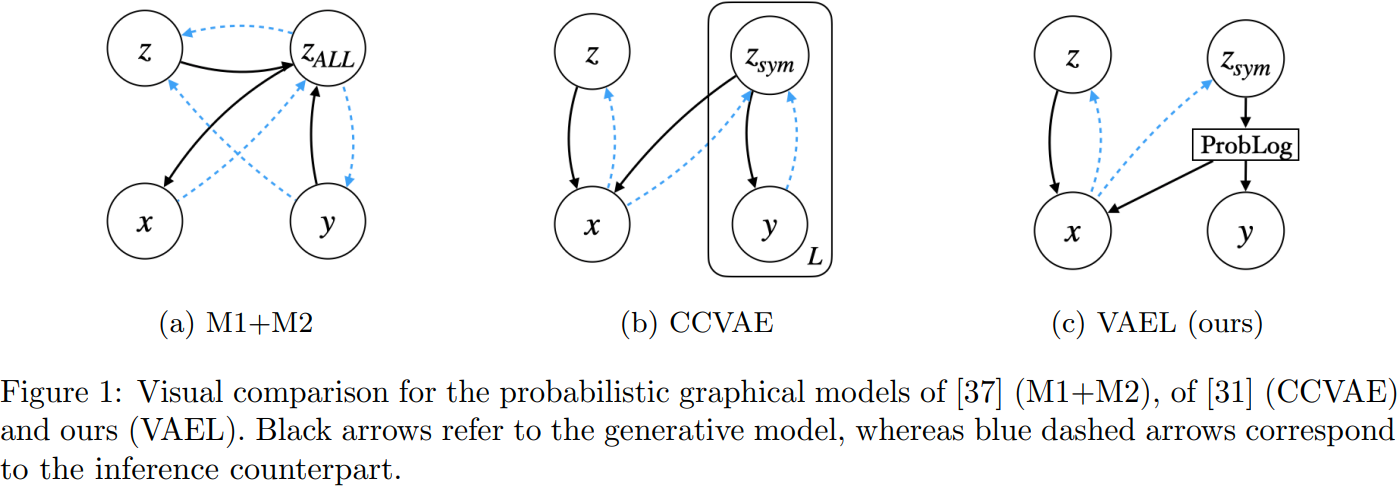
\includegraphics[width=0.95\textwidth]{figures/comparison.png}
        % \caption{}
        \label{fig:comparison}
    \end{figure}
    \begin{itemize}
        \item Model (M1+M2) learns a latent representation that is closely tied to the label, making the image generation dependent on the training task.
        \item The CCVAE model learns two independent latent vectors, one symbolic ($z_{\text {sym}}$) and one subsymbolic ($z$), with $z_{\text {sym}}$ directly corresponding to the label elements.
    \end{itemize}
}


\frame{
    \frametitle{Generation Conditioned on Labels (2)}
    \begin{figure}[htb]
        \centering
        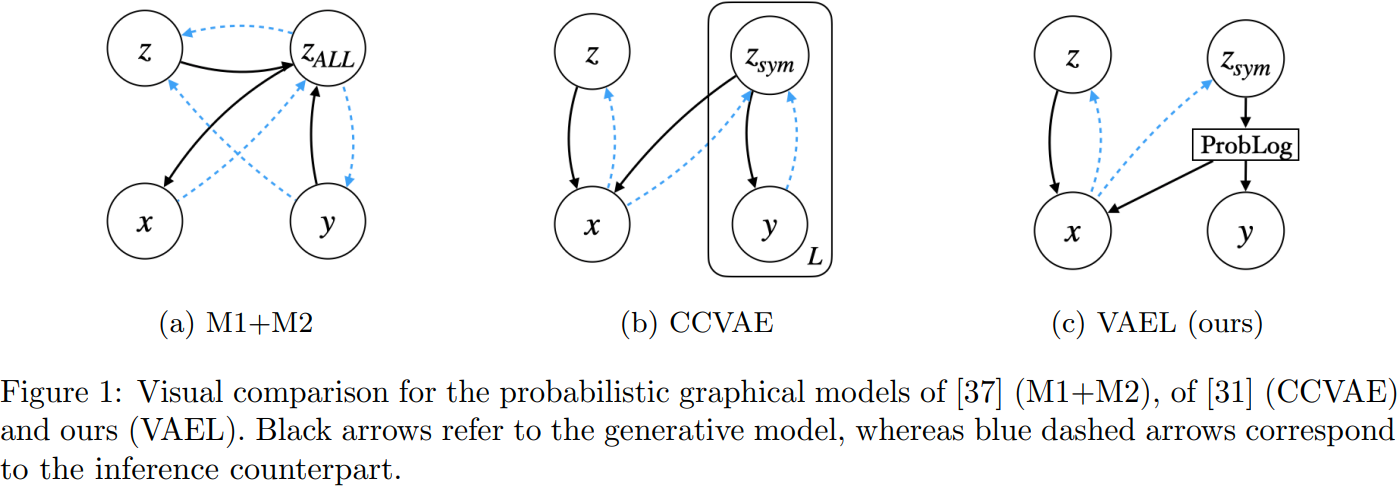
\includegraphics[width=0.95\textwidth]{figures/comparison.png}
        % \caption{}
        \label{fig:comparison}
    \end{figure}
    \begin{itemize}
        \item These methods are limited because they encode the training task into the latent representation, which is not ideal when the label is only weakly related to the image’s symbolic structure.
        \item How can we generate new images that represent different relationships between digits (like subtraction or multiplication) without retraining on new data, given that existing models are not capable of this flexibility?
    \end{itemize}
}



\section{Proposed Solution}

% 3. The VAEL Model
% Generative model
% Inference model

% \begin{itemize}
%     \item Model
%     \item Cost
%     \begin{itemize}
%         \item Required data
%         \item Required hardware
%         \item Complexity
%         \item \dots
%     \end{itemize}
% \end{itemize}

\frame{
    \subsection{The VAEL Model}
    \frametitle{The VAEL Model (1)} 
    The VAEL model integrates three main components: an encoder, a ProbLog program, and a decoder.
    \begin{figure}[htb]
        \centering
        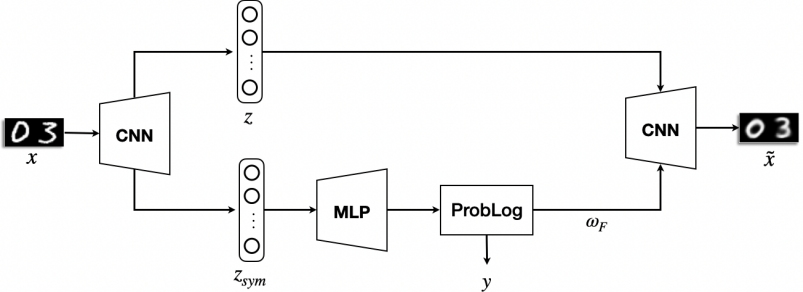
\includegraphics[width=1\textwidth]{figures/vael-model.png}
    \end{figure}
    \begin{itemize}
        \item The \textbf{encoder} processes the image $x$ to produce an approximated posterior of latent variables $\mathbf{z}$, which are divided into subsymbolic $z$ and symbolic $z_{\text {sym}}$ parts.
    \end{itemize}
}

\frame{
    \frametitle{The VAEL Model (2)} 
    \begin{figure}[htb]
        \centering
        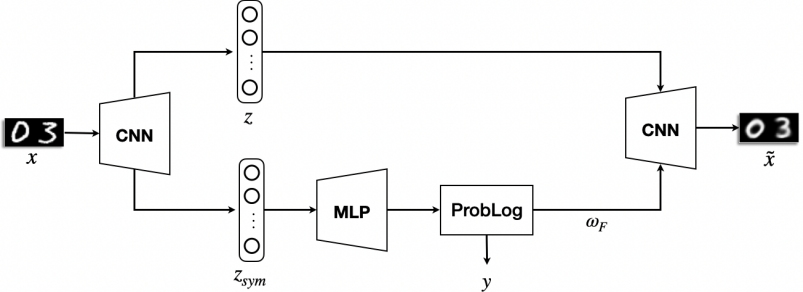
\includegraphics[width=1\textwidth]{figures/vael-model.png}
    \end{figure}
    \begin{itemize}
        \item The symbolic part, $z_{\text {sym}}$, parameterizes a \textbf{ProbLog program} that maps these variables to probabilities, which are then used to compute the label $y$ and a possible world.
        \item The \textbf{decoder} uses both the subsymbolic latent vector $z$ and the possible world from the ProbLog program to reconstruct the image $\tilde{x}$.
    \end{itemize}
}

\frame{
    \frametitle{The VAEL Model (3)} 
    \begin{figure}[htb]
        \centering
        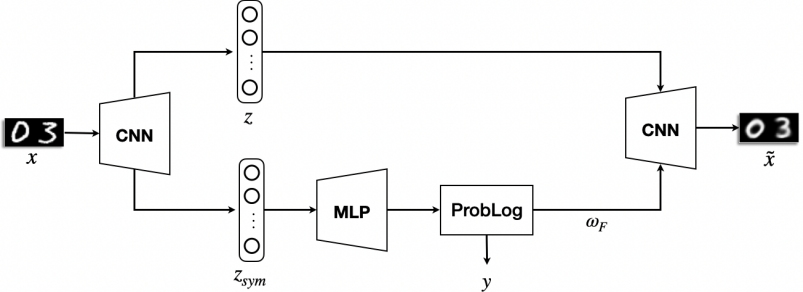
\includegraphics[width=1\textwidth]{figures/vael-model.png}
    \end{figure}
    The four core variables in this model are
    \begin{itemize}
        \item $x \in \mathbb{R}^{H \times W \times C}$: image we want to generate.
        \item $y \in\{0,1\}^{K}$: label (symbolic information characterizing the image).
        \item $z_{\text {sym}} \in \mathbb{R}^{N}$: symbolic component of the latent variable.
        \item $z \in \mathbb{R}^{M}$: subsymbolic component of the latent variable.
    \end{itemize}
}


\frame{
    \frametitle{Generative Model} 
    \begin{minipage}{0.72\textwidth}
        The generative distribution of VAEL is factorized as
        $$
            p_{\theta}(x, y, \mathbf{z}) =
            p(x \mid \mathbf{z}) p\left(y \mid z_{\text {sym}}\right) p(\mathbf{z})
        $$
        \begin{itemize}
            \item $\mathbf{z}=\left[z_{\text {sym }}, z\right]$
            \item $\theta$ are the parameters of the generative model
            \item $p(\mathbf{z})$ is a standard Gaussian distribution
            \item $p\left(y \mid z_{\text {sym}}\right)$ is the success distribution of the label of the ProbLog program $T$ 
            (\textcolor{black!60}{success probability})
            \item $p(x \mid \mathbf{z})$ is a Laplace distribution with mean value $\mu$ and identity covariance%, i.e. Laplace $(x ; \mu, I)$
            \item $\mu$ is a neural network decoder whose inputs are $z$ and $\omega_{F}$, which is sampled from $P\left(\omega_{F} ; M L P\left(z_{\text {sym}}\right)\right)$ 
            (\textcolor{black!60}{probability of a world})
        \end{itemize}
    \end{minipage}
    \begin{minipage}{0.26\textwidth}
        \begin{figure}[htb]
            \centering
            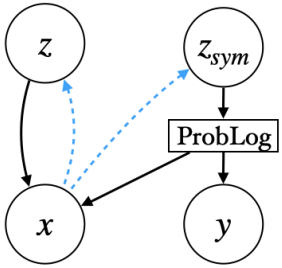
\includegraphics[width=1\textwidth]{figures/vael-graphical-model.png}
        \end{figure}
    \end{minipage}
}


\frame{
    \frametitle{Inference Model} 
    \begin{minipage}{0.72\textwidth}
        \begin{itemize}
            \item We amortize inference by using an approximate posterior distribution $q_{\phi}(\mathbf{z} \mid x,y)$.
            \item We assume that $\mathbf{z}$ and $y$ are conditionally independent given $x$
            $$
            q_{\phi}(\mathbf{z} \mid x, y)=q_{\phi}(\mathbf{z} \mid x)
            $$
            using a Gaussian distribution with mean parametrized by the encoder, and identity covariance.
            \item This allows to decouple the latent representation from the training task (unlike other VAE frameworks).
        \end{itemize}
    \end{minipage}
    \begin{minipage}{0.26\textwidth}
        \begin{figure}[htb]
            \centering
            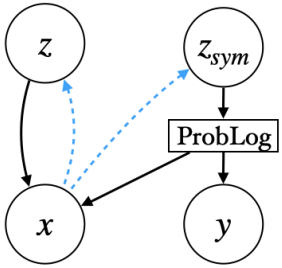
\includegraphics[width=1\textwidth]{figures/vael-graphical-model.png}
        \end{figure}
    \end{minipage}
}




\section{Model Validation}

% Objective function
% 4. Experiments

% \begin{itemize}
%     \item Mathematical proof
%     \item Experimental evaluation
% \end{itemize}

\frame{
    \frametitle{Objective Function}
    \subsection{Objective Function}
    The objective function of VAEL computes an ELBO on the log likelihood of pair $(x, y)$

    \begin{equation*}
        \mathcal{L}(\theta, \phi) =
        \textcolor{ForestGreen}{\mathcal{L}_{R E C}(\theta, \phi)} +
        \textcolor{Plum}{\mathcal{L}_{Q}(\theta, \phi)} -
        \mathcal{D}_{\mathcal{K} \mathcal{L}}\left[q_{\phi}(\mathbf{z} \mid x) \| p(\mathbf{z})\right]
    \end{equation*}\medskip

    \textcolor{ForestGreen}{Reconstruction error}
    $$
        \textcolor{ForestGreen}{\mathcal{L}_{R E C}(\theta, \phi)} =
        \mathbb{E}_{\mathbf{z} \sim q_{\phi}(\mathbf{z} \mid x)}\left[\log (p(x \mid \mathbf{z})\right]
    $$

    \textcolor{Plum}{Query error}
    $$
        \textcolor{Plum}{\mathcal{L}_{Q}(\theta, \phi)} =
        \mathbb{E}_{\left.z_{\text {sym}} \sim q_{\phi}\left(z_{\text {sym}} \mid x\right)\right)}\left[\log \left(p\left(y \mid z_{\text {sym}}\right)\right)\right]
    $$
}


\begin{frame}
    \frametitle{ELBO derivation (1)}
    Maximization of the log-likelihood of the input $x$ and the class $y$
    $$
        \log (p(x, y))=\log \left(\int p(x, y \mid \mathbf{z}) d \mathbf{z}\right)
    $$
    Recalling the generative network factorization $p(x, y, \mathbf{z})=p(x \mid \mathbf{z}) p(y \mid z_{\text {sym}}) p(\mathbf{z})$ we can write
    $$
        \log (p(x, y)) =
        \log \left(\int p_{\theta}\left(x \mid z, z_{\text {sym}}\right) p_{\theta}\left(y \mid z_{\text {sym}}\right) p(z) p\left(z_{\text {sym}}\right) d z d z_{\text {sym}}\right)
    $$
    The posterior $p_{\theta}(\mathbf{z} \mid x)$ is intractable, so we use the approximation $q_{\phi}(\mathbf{z} \mid x)$
    {\small
    \begin{multline*}
        \hspace{-0.35cm}\log (p(x, y))=\\
        \log \left(\int \frac{q_{\phi}(z \mid x) q_{\phi}\left(z_{\text {sym}} \mid x\right)}{q_{\phi}(z \mid x) q_{\phi}\left(z_{\text {sym}} \mid x\right)} p_{\theta}\left(x \mid z, z_{\text {sym}}\right) p_{\theta}\left(y \mid z_{\text {sym}}\right) p(z) p\left(z_{\text {sym}}\right) d z d z_{\text {sym}}\right)
    \end{multline*}
    }
\end{frame}


\begin{frame}
    \frametitle{ELBO derivation (2)}
    {\small
    $$
        \log \left(\int \frac{q_{\phi}(z \mid x) q_{\phi}\left(z_{\text {sym}} \mid x\right)}{q_{\phi}(z \mid x) q_{\phi}\left(z_{\text {sym}} \mid x\right)} p_{\theta}\left(x \mid z, z_{\text {sym}}\right) p_{\theta}\left(y \mid z_{\text {sym}}\right) p(z) p\left(z_{\text {sym}}\right) d z d z_{\text {sym}}\right)
    $$
    }
    By Jensen's inequality
    {\small
    $$
        \hspace{-0.5cm}\int q_{\phi}(z \mid x) q_{\phi}\left(z_{\text {sym}} \mid x\right) \log \left(p_{\theta}\left(x \mid z, z_{\text {sym}}\right) p_{\theta}\left(y \mid z_{\text {sym}}\right) \frac{p(z) p\left(z_{\text {sym}}\right)}{q_{\phi}(z \mid x) q_{\phi}\left(z_{\text {sym}} \mid x\right)} d z d z_{\text {sym}}\right)
    $$
    }
    This is the lower bound for the log-likelihood of $x$ and $y$, that can be rewrited as
    \begin{multline*}
        \mathbb{E}_{\mathbf{z} \sim q_{\phi}(\mathbf{z} \mid x)}\left[\log \left(p_{\theta}(x \mid \mathbf{z})\right)\right] ~
        + ~ \mathbb{E}_{z_{\text {sym}} \sim q_{\phi}\left(z_{\text {sym}} \mid x\right)}\left[\log \left(p_{\theta}\left(y \mid z_{\text {sym}}\right)\right)\right]\\
        + ~ \mathbb{E}_{\mathbf{z} \sim q_{\phi}(\mathbf{z} \mid x)}\left[\log \left(\frac{p(\mathbf{z})}{q_{\phi}(\mathbf{z} \mid x)}\right)\right]
    \end{multline*}
\end{frame}


\begin{frame}
    \frametitle{ELBO derivation (3)}
    \begin{multline*}
        \mathbb{E}_{\mathbf{z} \sim q_{\phi}(\mathbf{z} \mid x)}\left[\log \left(p_{\theta}(x \mid \mathbf{z})\right)\right] ~
        + ~ \mathbb{E}_{z_{\text {sym}} \sim q_{\phi}\left(z_{\text {sym}} \mid x\right)}\left[\log \left(p_{\theta}\left(y \mid z_{\text {sym}}\right)\right)\right]\\
        + ~ \mathbb{E}_{\mathbf{z} \sim q_{\phi}(\mathbf{z} \mid x)}\left[\log \left(\frac{p(\mathbf{z})}{q_{\phi}(\mathbf{z} \mid x)}\right)\right]
    \end{multline*}
    The last term is the negative KL divergence between the approximate posterior $q_{\phi}(\mathbf{z} \mid x)$ and the prior $p(\mathbf{z})$.
    This leads us to the ELBO of the objective function
    $$
    \def\arraystretch{1.5}
    \begin{array}{lclr}
        \log (p(x, y)) & \geq & \mathbb{E}_{\mathbf{z} \sim q_{\phi}(\mathbf{z} \mid x)}\left[\log \left(p_{\theta}(x \mid \mathbf{z})\right)\right] & \textcolor{ForestGreen}{\mathcal{L}_{R E C}(\theta, \phi)}\\
        & & + ~ \mathbb{E}_{z_{\text {sym}} \sim q_{\phi}\left(z_{\text {sym}} \mid x\right)}\left[\log \left(p_{\theta}\left(y \mid z_{\text {sym}}\right)\right)\right] & \textcolor{Plum}{\mathcal{L}_{Q}(\theta, \phi)}\\
        & & - ~ \mathcal{D}_{\mathcal{K} \mathcal{L}}\left[q_{\phi}(\mathbf{z} \mid x) \| p(\mathbf{z})\right] \\
        & :=  & \mathcal{L}(\theta, \phi)
    \end{array}
    $$
\end{frame}


\begin{frame}
    \frametitle{ELBO derivation (4)}
    In VAEL graphical model, $\omega_{F}$ is omitted since the authors exploit an equivalence relation between the probabilistic graphical models (PGMs). The objective for the PGM where $\omega_{F}$ is explicit (right) is equivalent to the one reported in the paper (left).

    \begin{figure}[htb]
        \centering
        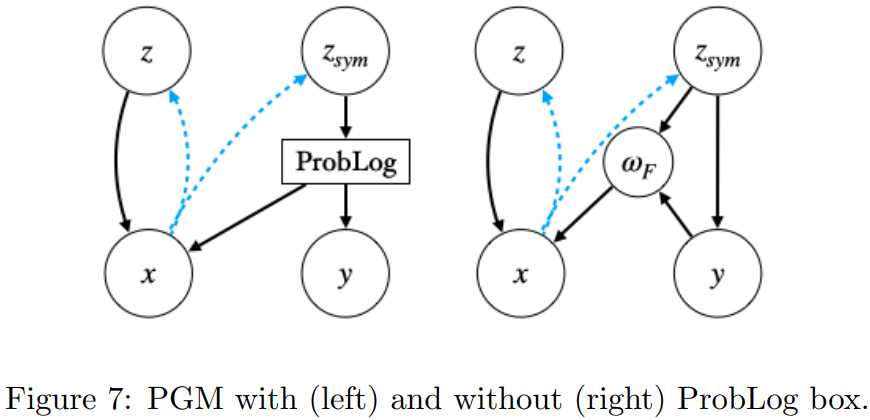
\includegraphics[width=0.8\textwidth]{figures/pgms.png}
        % \caption{}
        \label{fig:pgms}
    \end{figure}
\end{frame}


\begin{frame}
    \subsection{Training}
    \frametitle{Training (1)}
    \begin{itemize}
        \item The ELBO and its gradients were estimated w.r.t.~the model parameters using standard Monte Carlo estimates of expectations.
        \item Since both $q_{\phi}(\mathbf{z} \mid x)$ and $p(\mathbf{z})$ are chosen to be Gaussian distributions, the KL divergence in the objective function can be integrated analytically by relying on its closed form.
        \item Only the expected errors \textcolor{ForestGreen}{$\mathcal{L}_{R E C}(\theta, \phi)$} and \textcolor{Plum}{$\mathcal{L}_{Q}(\theta, \phi)$} require estimation by sampling.
    \end{itemize}\medskip

    \noindent ELBO estimator:
    $$
        \mathcal{L}(\theta, \phi) \approx \tilde{\mathcal{L}}(\theta, \phi ; \epsilon)=
        \textcolor{Emerald}{\tilde{\mathcal{L}}_{R E C}(\theta, \phi ; \epsilon)}+
        \textcolor{RubineRed}{\tilde{\mathcal{L}}_{Q}(\theta, \phi ; \epsilon)}-
        \mathcal{D}_{\mathcal{K} \mathcal{L}}\left[q_{\phi}(\mathbf{z} \mid x) \| p(\mathbf{z})\right]
    $$
\end{frame}


\begin{frame}
    \frametitle{Training (2)}
    $$
        \mathcal{L}(\theta, \phi) \approx \tilde{\mathcal{L}}(\theta, \phi ; \epsilon)=
        \textcolor{Emerald}{\tilde{\mathcal{L}}_{R E C}(\theta, \phi ; \epsilon)}+
        \textcolor{RubineRed}{\tilde{\mathcal{L}}_{Q}(\theta, \phi ; \epsilon)}-
        \mathcal{D}_{\mathcal{K} \mathcal{L}}\left[q_{\phi}(\mathbf{z} \mid x) \| p(\mathbf{z})\right]
    $$

    \textcolor{Emerald}{Estimated reconstruction error}
    $$
        \textcolor{Emerald}{\tilde{\mathcal{L}}_{R E C}(\theta, \phi ; \epsilon)} =
        \frac{1}{N} \sum_{n=1}^{N}\left(\log \left(p_{\theta}\left(x \mid \hat{\mathbf{z}}^{(n)}\right)\right)\right)
    $$

    \textcolor{RubineRed}{Estimated query error}
    $$
        \textcolor{RubineRed}{\tilde{\mathcal{L}}_{Q}(\theta, \phi ; \epsilon)} =
        \frac{1}{N} \sum_{n=1}^{N}\left(\log \left(p_{\theta}\left(y \mid \hat{z}_{\text {sym }}^{(n)}\right)\right)\right)
    $$
    where
    $$
        \hat{\mathbf{z}}^{(n)} =\left\{\hat{z}^{(n)}, \hat{z}_{\text {sym}}^{(n)}\right\}:=\mu(x)+\sigma(x) \epsilon^{(n)} , \qquad
        \epsilon^{(n)} \sim \mathcal{N}(0,1)
    $$
\end{frame}


\begin{frame}
    \frametitle{Training (3)}
    \begin{itemize}
        \item During training, the aim is to maximize $\mathcal{L}(\theta, \phi)$ w.r.t~both the encoder and the decoder parameters: we need to compute the gradient w.r.t.~$\theta$ and $\phi$.
        \item Since any sampling operation prevents back-propagation, we need to reparametrize the two sampled variables $\mathbf{z}$ and $\omega$.
        \item The authors used for the Gaussian $\mathbf{z}$ the Reparametrization Trick, and for the discrete variable $\omega$ (corresponding to the sampled possible world) they exploited the Categorical Reparametrization with Gumbel-Softmax.
    \end{itemize}
\end{frame}


\begin{frame}
    \frametitle{Training (4)}
    \begin{figure}[htb]
        \centering
        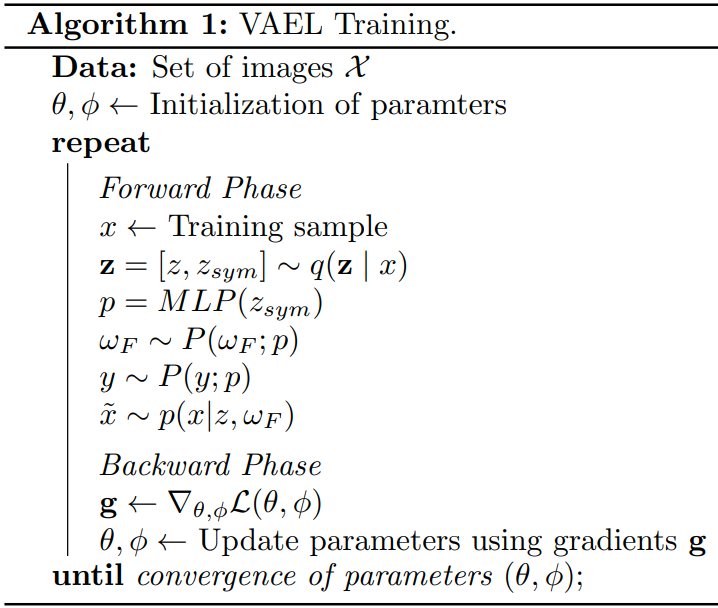
\includegraphics[width=0.75\textwidth]{figures/algorithm.png}
        % \caption{}
        \label{fig:algo}
    \end{figure}
    {\footnotesize
    $$
        P\left(w_{F} ; p\right)=\prod_{f_{i} \in F} p_{i} \prod_{f_{i} \in \mathcal{F} \backslash F}\left(1-p_{i}\right) \qquad\qquad
        P(y ; p)=\sum_{F \subseteq \mathcal{F}: w_{F} \models y} P\left(w_{F} ; p\right)
    $$
    }
\end{frame}


\begin{frame}
    \subsection{Experiments}
    \frametitle{Experiments}
    \begin{itemize}
        \item \textbf{Datasets}: A 2digit MNIST dataset with 64,400 images and a Mario dataset with 6,720 images were created for testing.
        \item \textbf{Dataset Splits}: The 2digit MNIST dataset was split into 65\% training, 20\% validation, and 15\% test sets, while the Mario dataset was split into 70\% training, 20\% validation, and 10\% test sets.
        \item \textbf{Evaluation Metrics}: The approach was evaluated using reconstruction loss (mREC), predictive accuracy (mCLASS), and generative accuracy (mGEN).
        \item \textbf{Predictive Accuracy}: For the 2digit MNIST dataset, predictive accuracy is based on the sum of the two digits, and for the Mario dataset, it’s based on the agent’s move.
        \item \textbf{Generative Accuracy}: An independent classifier was used for each dataset to assess generative accuracy, which involves generating an image and label, splitting the image, classifying the parts, and comparing the results with the generated label.
        \item \textbf{Model Comparison}: VAEL was compared with CCVAE where possible.
    \end{itemize}
\end{frame}


\begin{frame}
    \frametitle{Label Classification}
    \begin{itemize}
        \item \textbf{Goal}: Predict the correct label from the input image, evaluated by predictive accuracy (mCLASS).
        \item \textbf{Method}: VAEL uses ProbLog inference, while CCVAE uses a neural network to parameterize ( $p(y|z_{\text{sym}})$ ).
        % \item Results: VAEL and CCVAE perform similarly on the Mario dataset but VAEL excels on the 2digit MNIST dataset due to its better handling of combinatorial nature tasks.
    \end{itemize}
    \begin{figure}[htb]
        \centering
        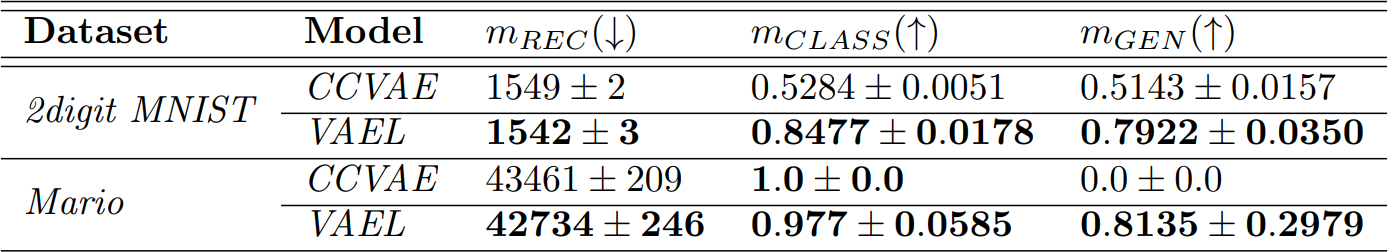
\includegraphics[width=1\textwidth]{figures/table.png}
    \end{figure}
\end{frame}


\begin{frame}[t]
    \frametitle{Image Generation}
    \begin{itemize}
        \item \textbf{Goal}: Assess model performance in generating both the image and its label.
        \item \textbf{Method}: VAEL generates from a sampled latent vector ($\mathbf{z} \sim \mathcal{N}(0, 1)$), while CCVAE samples a label first, then the latent vector, and finally the image.
        % \item Results: VAEL produces well-defined digits for the 2digit MNIST dataset and data-like images for the Mario dataset. CCVAE struggles with ambiguous digit generation and fails to draw the agent in the Mario dataset.
    \end{itemize}
    \begin{figure}[htb]
        \centering
        \begin{subfigure}[][0pt][t]{0.4\textwidth}
            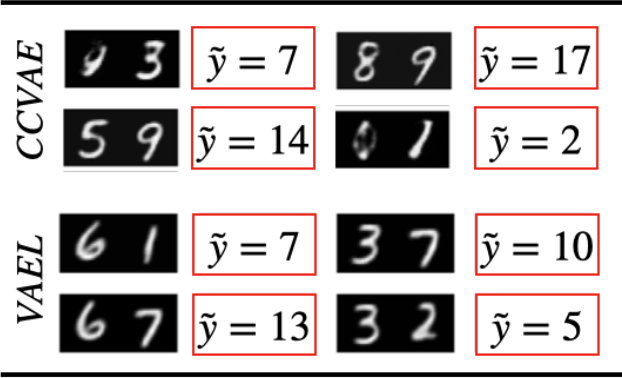
\includegraphics[width=\textwidth]{figures/img-gen.png}
        \end{subfigure}
        \hspace{1cm}
        \begin{subfigure}[][0pt][t]{0.3\textwidth}
            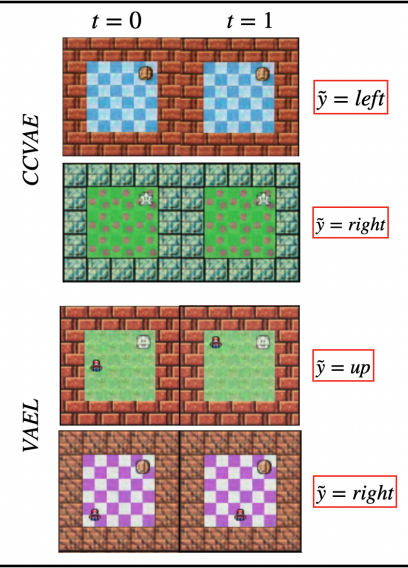
\includegraphics[width=\textwidth]{figures/img-gen2.png}
        \end{subfigure}
    \end{figure}
\end{frame}


\begin{frame}[t]
    \frametitle{Conditional Image Generation}
    \begin{itemize}
        \item \textbf{Goal}: Evaluate the model's ability to generate images conditionally based on evidence.
        \item \textbf{Method}: VAEL consistently generates coherent pairs of digits and states, while CCVAE often fails to meet the evidence criteria.
        % \item Results: VAEL shows versatility and accuracy in generating images that align with the given evidence, outperforming CCVAE, which exhibits limitations in task complexity.
    \end{itemize}
    \begin{figure}[htb]
        \centering
        \begin{subfigure}[][0pt][t]{0.45\textwidth}
            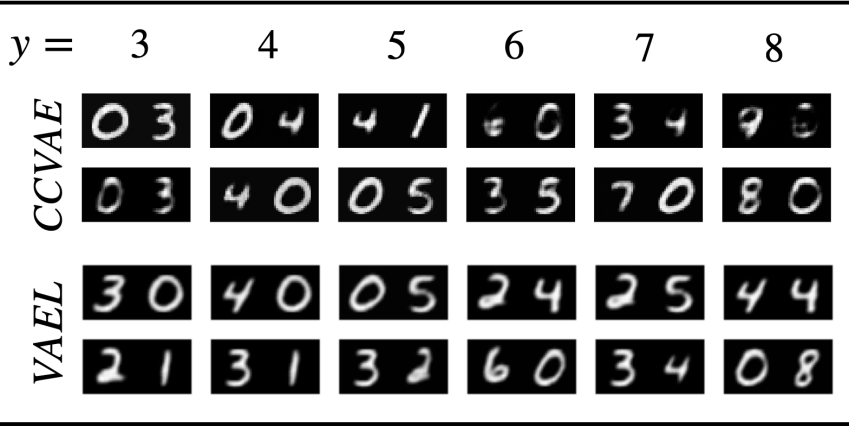
\includegraphics[width=\textwidth]{figures/cond-gen.png}
        \end{subfigure}
        \hfill
        \begin{subfigure}[][0pt][t]{0.5\textwidth}
            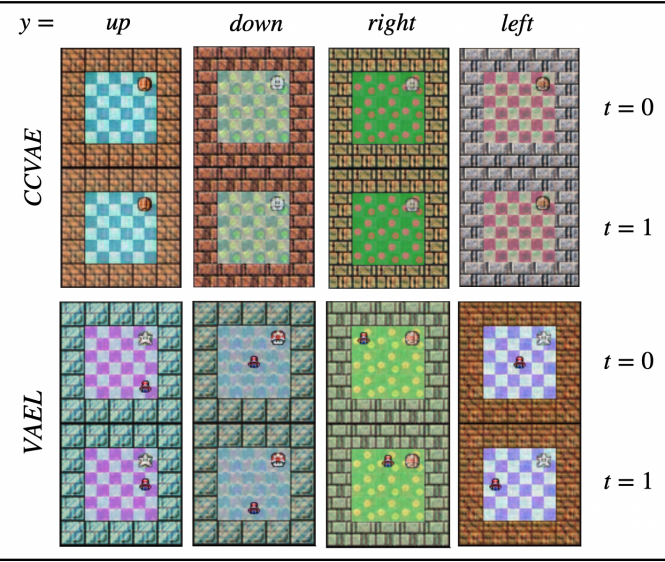
\includegraphics[width=\textwidth]{figures/cond-gen2.png}
        \end{subfigure}
    \end{figure}
\end{frame}


\begin{frame}[t]
    \frametitle{Task Generalization}
    \begin{itemize}
        \item \textbf{Goal}: Test VAEL’s ability to generalize to new tasks without retraining.
        \item \textbf{Approach}: For the 2digit MNIST dataset, tasks like multiplication, subtraction, and exponentiation were introduced. For the Mario dataset, two shortest path tasks were defined.
        % \item Results: VAEL successfully generalized to these new tasks by simply changing the ProbLog program, demonstrating its flexibility and robustness.
    \end{itemize}
    \begin{figure}[htb]
        \centering
        \begin{subfigure}[][0pt][t]{0.45\textwidth}
            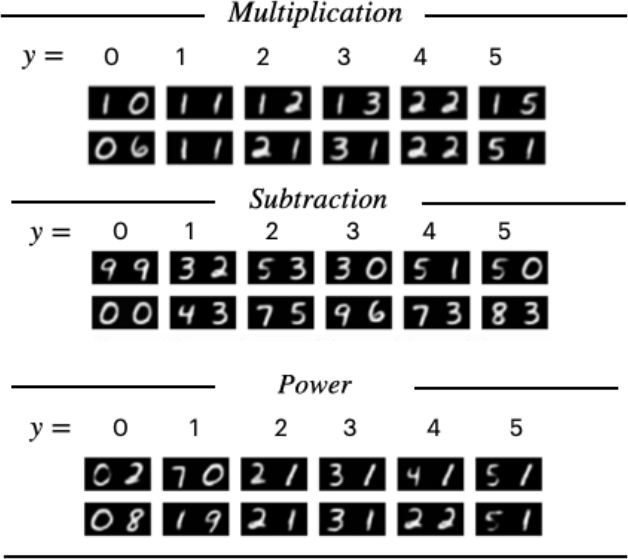
\includegraphics[width=\textwidth]{figures/generaliz.png}
        \end{subfigure}
        \hfill
        \begin{subfigure}[][0pt][t]{0.5\textwidth}
            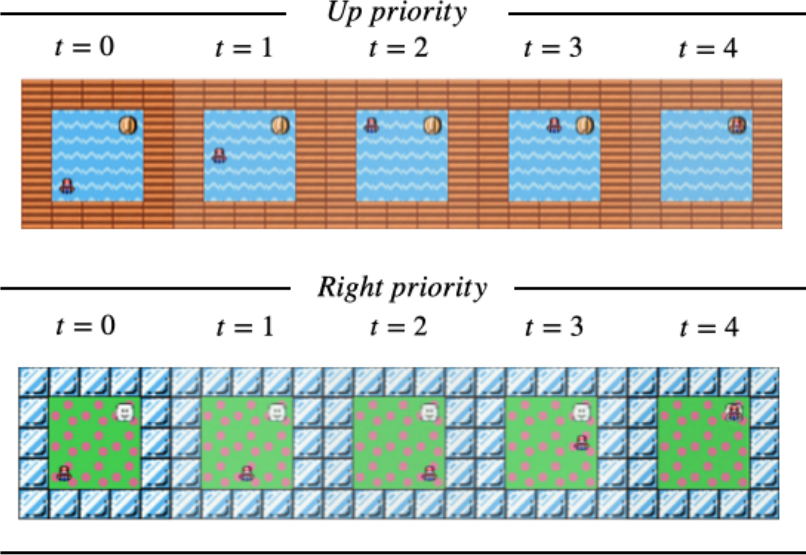
\includegraphics[width=\textwidth]{figures/generaliz2.png}
        \end{subfigure}
    \end{figure}
\end{frame}




% 5. Related Work
    
% \begin{itemize}
%     \item Differences with the literature
%     \item Strengths
%     \item Weaknesses
% \end{itemize}


\section{Critical Analysis}

\frame{
    \subsection{Related Work}
    \frametitle{Controlled Image Generation} 
    \begin{itemize}
        \item Generative models are categorized into those based on \textbf{text descriptions} and those using \textbf{scene graphs}.
        \item \textbf{Text-based models} focus on controlling \emph{object properties} (shape, color, texture), \emph{spatial relations} (positioning of objects relative to each other), or \emph{both properties and relations}.
        % \item This paper's framework relates to these models by addressing image generation in a relational context.
        \item Unlike previous works, VAEL framework employs probabilistic logic programming to encode and reason with first-order logical knowledge.
        \item This method allows for generalization to both compositions of known relations and entirely new relations.
        \item \textbf{Scene graph-based models} explicitly encode object relations but are less expressive than the logical programs used in this framework, which enable more general reasoning capabilities.
    \end{itemize}
}


\frame{
    \frametitle{Unsupervised Scene Decomposition} 
    Unsupervised scene decomposition is categorized into:
    \begin{itemize}
        \item \textbf{Object-oriented approaches}: Focus on learning representations of individual objects to reconstruct images or sequences.
        \item \textbf{Part-oriented approaches}: Decompose objects into their basic parts for reconstruction.
        \item \textbf{Hierarchical approaches}: Combine the above two to decompose scenes into objects and their parts.
    \end{itemize}
    \textbf{Current Methods} use scene-mixtures, spatial attention models, and combinations for \emph{object-oriented decomposition}, and employ encoders and decoders for \emph{part-oriented decomposition}. Recent efforts aim to achieve \emph{hierarchical decomposition}, learning both objects and parts.\smallskip 

    \textbf{This paper's approach} focuses on static images, not using temporal information. Does not rely on predefined information about object locations. Utilizes a simple autoencoder architecture to discover objects based on logical relations. 
    % Presents a different direction that could benefit from advancements in unsupervised scene decomposition in future work. 
}


\frame{
    \frametitle{Neuro-Symbolic Generation} 
    \begin{itemize}
        \item Neuro-symbolic generation is a new field combining machine learning with logical reasoning.
        \item Previous models had a two-layered latent representation for scenes and objects but were limited to specific spatial relations.
        \item VAEL model uses a \textbf{logical reasoning framework} to handle a wider range of generative tasks and knowledge manipulation.
        \item Attempts to integrate generative models with probabilistic programming have been made, but they often had limited reasoning capabilities.
        \item This paper's approach provides a \textbf{unified model} that can generate images and perform logical reasoning simultaneously.
        % \item The work cited as [60] was an early attempt to combine generative models with logic, but it had limitations in application and integration.
        % The authors of the paper have developed a probabilistic graphical model that integrates the symbolic and perceptual aspects more effectively.
        \item The authors are the first to conduct experiments showing the \textbf{benefits of this integration} in terms of task generalization and data efficiency.
    \end{itemize}
}


\frame{
    \frametitle{Neuro-Symbolic Generation} 
    \begin{itemize}
        \item Neuro-symbolic generation is a new field combining machine learning with logical reasoning.
        \item Previous models had a two-layered latent representation for scenes and objects but were limited to specific spatial relations.
        \item VAEL model uses a \textbf{logical reasoning framework} to handle a wider range of generative tasks and knowledge manipulation.
        \item Attempts to integrate generative models with probabilistic programming have been made, but they often had limited reasoning capabilities.
        \item This paper's approach provides a \textbf{unified model} that can generate images and perform logical reasoning simultaneously.
        % \item The work cited as [60] was an early attempt to combine generative models with logic, but it had limitations in application and integration.
        % The authors of the paper have developed a probabilistic graphical model that integrates the symbolic and perceptual aspects more effectively.
        \item The authors are the first to conduct experiments showing the \textbf{benefits of this integration} in terms of task generalization and data efficiency.
    \end{itemize}
}


\section{Conclusions}

\frame{
    \frametitle{Conclusions} 
    \begin{itemize}
        \item \textbf{VAEL Model}: Introduced as a neuro-symbolic generative model combining Variational Autoencoders (VAE) with Probabilistic Logic Programming.
        \item \textbf{Symbolic Component}: Enables the model to separate its internal understanding from specific tasks, leading to powerful generalization capabilities.
        \item \textbf{Performance}: Demonstrated state-of-the-art image generation abilities in benchmarks, excelling even with limited data and across various prediction tasks.
        \item \textbf{Future Improvements}: Plans to explore more scalable options for probabilistic programs, such as stochastic logic programs.
        \item \textbf{Broader Applications}: Aims to apply VAEL in different domains like structured object generation to further demonstrate its flexibility and expressiveness.
    \end{itemize}
}


\frame{
    % \frametitle{Conclusions}
    \begin{center}
        \Huge \textbf{Thank you!}
    \end{center} 
    \vfill 
    All material and images can be found in the original paper
    \url{https://papers.nips.cc/paper_files/paper/2022/hash/1e38b2a0b77541b14a3315c99697b835-Abstract-Conference.html}
}


\end{document}